\documentclass[11pt]{scrartcl}
\usepackage[utf8]{inputenc}
\usepackage{enumitem}
\usepackage{amsfonts}
\usepackage{bbm}
\usepackage{newtxmath}
%\usepackage[square]{natbib}
\usepackage{amsmath}
\usepackage{mathrsfs,bm}
\usepackage{graphicx,epstopdf,caption}
\usepackage{float,subcaption,setspace,booktabs,multirow,supertabular,lscape,threeparttable}
\usepackage{float,colortbl}
\usepackage{placeins}
\usepackage{indentfirst}
\usepackage{enumitem}
\setlength{\parindent}{0pt} %% noindent for the entire file % or add indent {2em}
\usepackage{geometry}
\geometry{left=0.8in,right=0.8in,top=1in,bottom=0.5in}
\usepackage[noblocks]{authblk}
\usepackage{lipsum}%% a garbage package you don't need except to create examples.
\usepackage{fancyhdr}
\usepackage[svgnames]{xcolor}
\usepackage{listings}
\usepackage{verbatim}
\usepackage[round, semicolon, sort]{natbib}
\setlength{\parindent}{2em}
%\setlength{\parskip}{0.5em}

\pagestyle{fancy}
\lhead{CSCI 5561}  % set your name here
\chead{\large\textbf{Homework 1 - HOG}}
\rhead{He Zhou (zhou1354@umn.edu)}
\renewcommand{\headrulewidth}{0.4pt}

\lstset{language=R,
	basicstyle=\small\ttfamily,
	stringstyle=\color{DarkGreen},
	otherkeywords={0,1,2,3,4,5,6,7,8,9},
	morekeywords={TRUE,FALSE},
	deletekeywords={data,frame,length,as,character},
	keywordstyle=\color{blue},
	commentstyle=\color{DarkGreen},
}
\usepackage{Sweave}
\graphicspath{{Figures/}}  % set the path of figures
\usepackage{blindtext}
\usepackage{scrextend}
\addtokomafont{labelinglabel}{\bfseries}
\usepackage{appendix}
\usepackage[linesnumbered,ruled,vlined]{algorithm2e}

\usepackage{algpseudocode}  
\usepackage{hyperref}
\hypersetup{
    colorlinks=true,
    linkcolor=blue,
    filecolor=blue,      
    urlcolor=blue,
    citecolor=cyan,
}

\newcommand{\cX}{\mathcal{X}}
\newcommand{\cR}{\mathcal{R}}
\newcommand{\cV}{\mathcal{V}}
\newcommand{\bw}{\mathbf{w}}

	

\begin{document}

\title{CSCI 5561}
\author{\Large Homework 1 -- HOG\\
	He Zhou}  %% set your name on the main page
%\date{\vspace{-5ex}}  % suppress the output of date
\maketitle

\newpage
\noindent\textbf{HOG }\quad
In this assignment, a variant of HOG proposed by \cite{dalal2005histograms} is implemented. We follow the Algorithm 1 (\texttt{extract\_hog}) for computing the HOG descriptor:

(1) \texttt{get\_differential\_filter}: Get the sobel differential filters:
\begin{equation*}
	\texttt{filter\_x}=\begin{pmatrix}
	-1&0&1\\-2&0&2\\-1&0&1
	\end{pmatrix},\quad
	\texttt{filter\_y}=\begin{pmatrix}
		-1&-2&-1\\0&0&0\\1&2&1
	\end{pmatrix}.
\end{equation*}

(2) \texttt{filter\_image}: Compute the gradient along $x$ and $y$ directions. Zeros are padded on the boundary on the input image to get the same size filtered image.

(3) \texttt{get\_gradient}: Compute the magnitude and angle of the gradient. The range of the angle is $[0,\pi)$, i.e., for $\theta\in[-\pi,0)$, set $\theta=\theta+\pi$; for $\theta=\pi$, set 
$\theta=0$.

(4) \texttt{build\_histogram}: Divide the image to cells based on the \texttt{cell\_size} (typical is 8). Build the histogram of oriented gradients for each cell with the $6$ bins given by $\theta_1=[165, 180)\cup[0, 15)$, $\theta_2=[15,45)$, $\theta_3=[45,75)$, $\theta_4=[75,105)$, $\theta_5=[105,135)$, $\theta_6=[135,165)$.

(5) \texttt{get\_block\_descriptor}: HOG is locally normalized to account for changes in illumination and contrast. Group the cells together into larger, spatially connected blocks (use \texttt{block\_size}=2) and apply $L_2$ normalization to the descriptor ($e=0.001$).

Figure \ref{fig:cameraman_HOG} shows the figure of visualizing the HOG discriptor of the \texttt{`cameraman.tif'} image using the \texttt{visualize\_hog} function.
\\
\textbf{Application: Face Detection}\quad By using the HOG descriptor, we can use a simgle template image \texttt{`template.png'} ($50\times50$) to detect faces in the target image \texttt{`target.png'} ($135\times240$). First, measure the \textbf{normalized cross-corrlation (NCC)} between the HOG descriptors from the template and target image patches. Then \textbf{thresholding} on NCC scores using threshold value $0.48$, i.e., all the bounding boxes with NCC scores $<0.48$ will be deleted. As thresholding will produce many overlapping bouding boxes, we use \textbf{non-maximum suppression} with IoU 50\% to detect correct bounding boxes for faces.

We need to compute the HOG descriptors of all target patches, which is $(135-50+1)*(240-50+1)=16426$ patches in total. It took around 10 minutes to run the \texttt{face\_recognition} function. Figure \ref{fig:face_thresholding} shows the plot of visualizing the bounding boxes after thresholding on NCC scores. We can see many overlapping bounding boxes. Figure \ref{fig:face_nms} shows the plot of bounding boxes obtained by non-maximum suppression. We can see that all the five faces are correctly detected and each face is detected only once.



\begin{figure}[H]
	\centering
	\begin{subfigure}{0.5\textwidth}
		\centering
		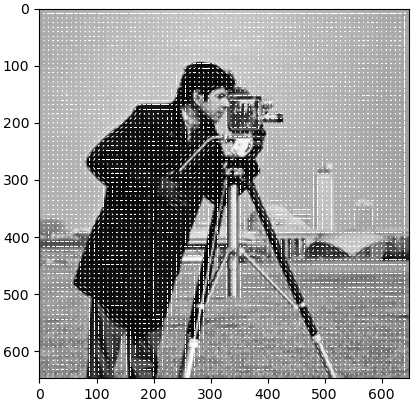
\includegraphics[scale=0.4]{cameraman_HOG.png}
		\caption{}
		\label{fig:cameraman_HOG}
	\end{subfigure}%
	\begin{subfigure}{0.5\textwidth}
		\centering
		\begin{minipage}{1\textwidth}
			\centering
			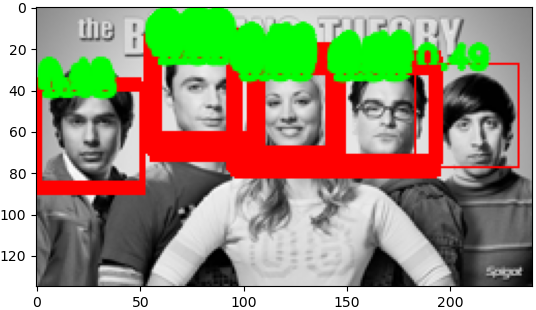
\includegraphics[scale=1]{face_thresholding.png}
			\caption{}
			\label{fig:face_thresholding}
		\end{minipage}
		\vspace{0.5in}
		\begin{minipage}{1\textwidth}
			\centering
			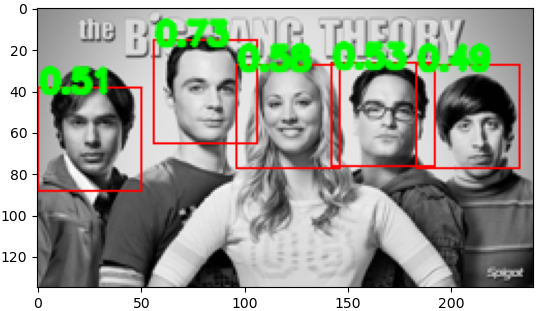
\includegraphics[scale=1]{face_nms.png}
			\caption{}
			\label{fig:face_nms}
		\end{minipage}
	\end{subfigure}
\end{figure}










\nocite*{}  
%\bibliographystyle{apalike}  %disordered
%\bibliographystyle{plain}  %ordered by auther
%\bibliographystyle{unsrt}  %ordered as referenced
\bibliographystyle{IEEEtranN}
\bibliography{bibfile}






\end{document}